\section{Системы координат.}

Рассмотрим открытую кинематическую цепь состоящей из простых кинематических звеньев. С каждым кинематическим звеном свяжем две локальные системы координат, распожив их в точках сочленения кинематических пар. Таким образом каждое кинематическое звено имеет входную и выходную ЛСК, жестко связанные с ним.

В сочленении кинематической пары также оказывается две системы координат - по одной для каждого звена пары (выходная первого звена и входная второго). Введем кинематические параметры звеньев $q_i$, определяющих взаимное расположение локальных систем координат.

\begin{center}
  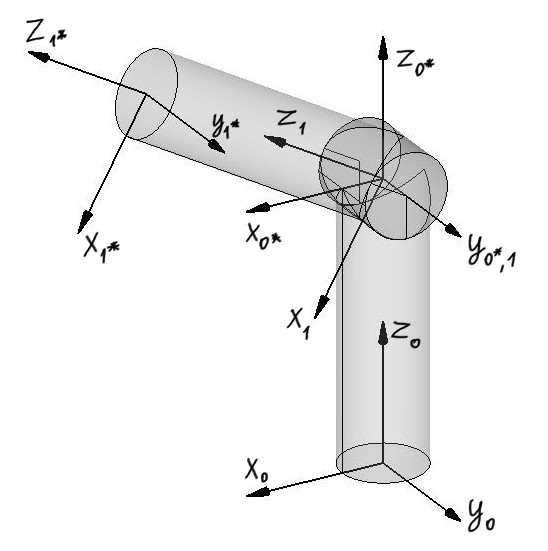
\includegraphics[width=0.6\textwidth,height=0.6\textheight,keepaspectratio]{ax3view.jpg}
  \captionof{figure}{Взаимное расположение систем координат для кинематического звена в виде поворотного шарнира.}
  \label{}
\end{center}

Таким образом кинематическая цепь определяется цепочкой локальных систем координат, положение каждой из которых определяется положением предыдущей и объектом гомогенного преобразования, либо константным, либо завищим от соответствующего кинематического параметра.

Пронумеруем звенья и системы координат. Пусть неподвижное кинематическое звено, жестко связанное с лабораторной системой координат считается 0-ым, лабораторная система координат считается 0-ой СК, пусть входная система каждого $n$-ого звена считается $n$-ой СК. Выходную систему кинематического звена обозначим как $n^*$. 

Если в нашей цепи $m$ звеньев, то СК выходного звена цепи будут иметь номера $m$ и $m*$.

Конкретный тип кинематического звена не имеет существенного значения в рамках метода, но желательно, чтобы объект гомогенного преобразования, связывающий системы координат $(n-1)*$ и $n$, зависел исключительно от обобщенных координат текущей кинематической пары.

Наиболее часто применяемым на практике является кинематическое звено в виде одностепенного поворотного шарнира с объектом преобразования:
\begin{equation}
H^i_{{i-1}^*} = |\rho, r| = |\phi|u_1, u_2, u_3|, |0, 0, 0||
\end{equation}, где $\phi$ - обобщенная координата.

Также интерес представляет актуаторное звено, реализующее линейное перемещение и имеющее объект преобразования:
\begin{equation}
H^i_{{i-1}^*} = |\rho, r| = ||0, 0, 0|, l|u_1, u_2, u_3||
\end{equation}, где $l$ - обобщенная координата.

\begin{center}
  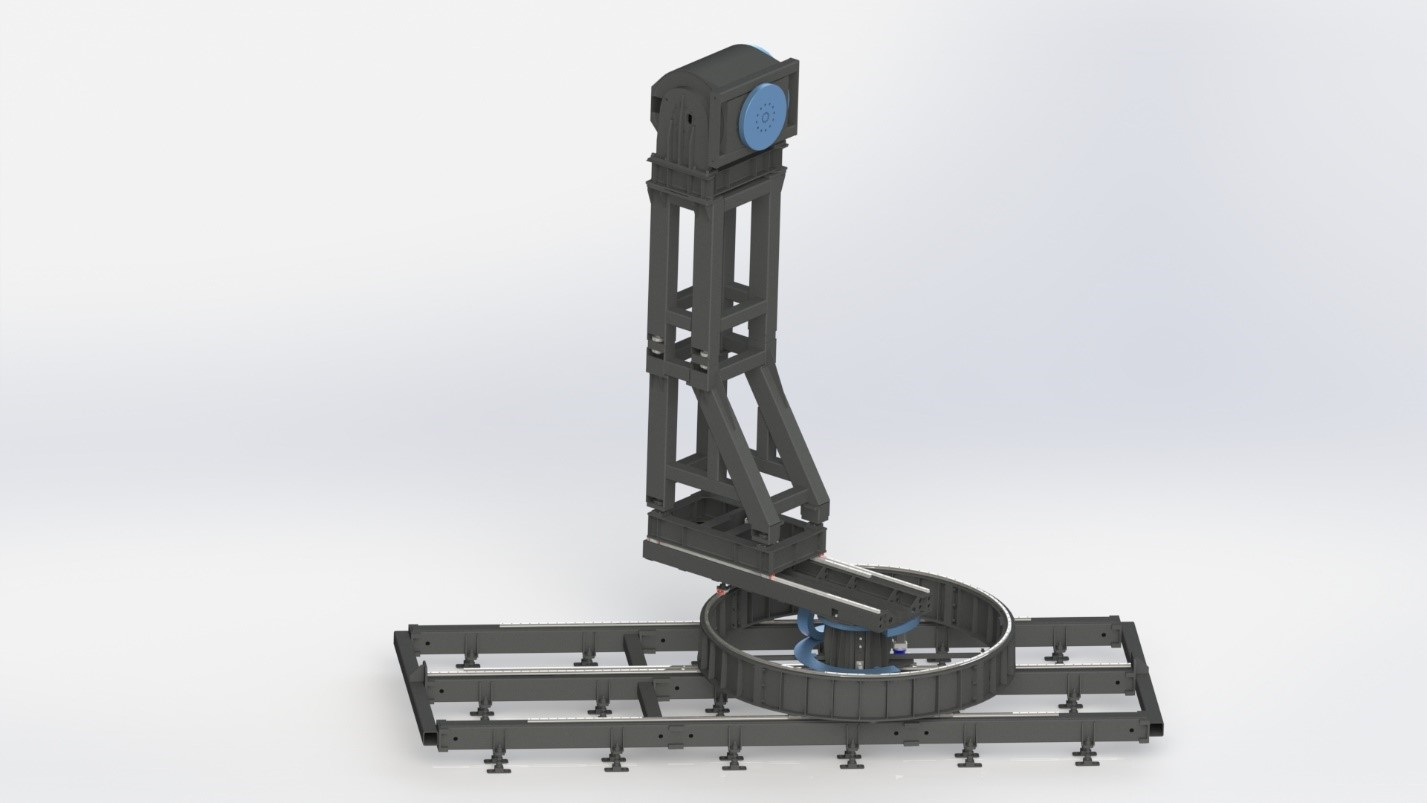
\includegraphics[width=0.6\textwidth,height=0.6\textheight,keepaspectratio]{actexample.jpg}
  \captionof{figure}{Пример системы с актуаторными кинематическими звеньями..}
  \label{}
\end{center}

\begin{center}
  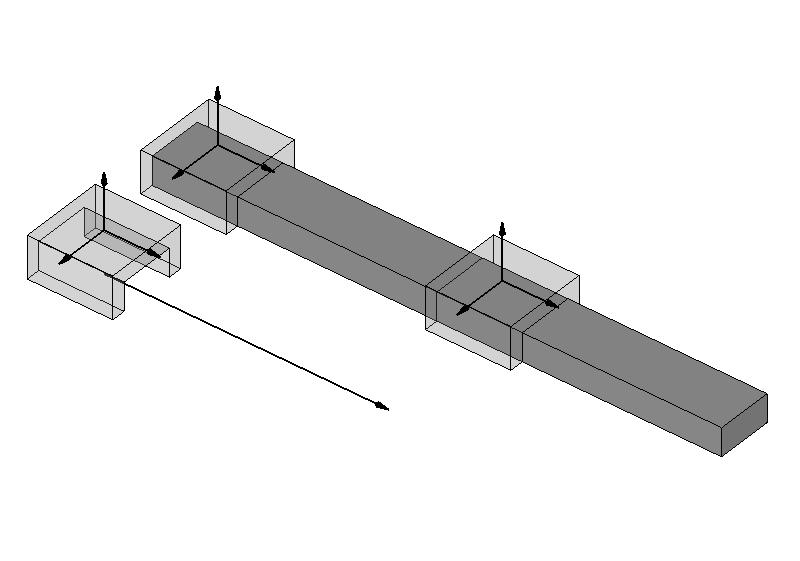
\includegraphics[width=0.6\textwidth,height=0.6\textheight,keepaspectratio]{actsyst.jpg}
  \captionof{figure}{Взаимное расположение систем координат для актуаторного кинематического звена.}
  \label{}
\end{center}

Введение иных кинематических звеньев также возможно, не нарушает вывода, но выходит за рамки настоящего изложения. Введение кинематических пар класса отличного от пятого, хотя и не рассматривается в данной работе не нарушает общности метода, поскольку всегда можно считать, что две или более координаты кинематической пары связаны звеном с единичным объектом преобразования $H^i_{{i-1}^*} = ||0, 0, 0| |0, 0, 0||$.